\documentclass[document.tex]{subfiles} 
\begin{document}
\clearpage\section{Описание программного решения}
\subsection{Разработка программной библиотеки}
Исходя из ограничений существующих решений, было решено в рамках проекта
реализовать свою библиотеку для синтеза цифровых комбинационных схем на языке
программирования Python с использованием библиотеки символьной алгебры логики
SymPy и библиотеки для работы с графами NetworkX.

Декомпозиция проекта при проектировании проведена таким образом, чтобы разделить
сущности устройств синтезируемых схем и адаптеров для отображения схем в
различных форматах. Независимость сущностей дает возможность применять
однотипные способы описания устройств к совершенно различным синтезированным
устройствам, построенным на единой парадигме символьной алгебры.

Для наглядной демострации функциональных возможностей разрабатываемой
библиотеки синтеза схемотехнических устройств, также был разработан интерфейс
пользователя на базе языка программирования Python с использованием фреймворка
Flask и языка программирования JavaScript с использованием фреймворка ExtJS 4.
Программное обеспечение представляет собой веб-приложение и может быть запущено с использованием сети
Интернет. Единственной особенностью связки с основной библиотекой
схемотехнического моделирования, является механизм интроспекции классов
устройств и классов адаптеров, автоматический импорт используемых сущностей и
унификация вывода информации в приложение.

\clearpage
\subsection{Графический интерфейс пользователя}
Основной интерфейс пользователя представляет собой таблицу с перечнем типов
устройств, синтез которых поддерживается библиотекой проекта, кнопку настройки сигналов
устройств, выпадающий список выбора адаптера и кнопку обработки.
На рисунке~\ref{fig:interface_index} представлена заглавная страница интерфейса.

\begin{figure}[here]
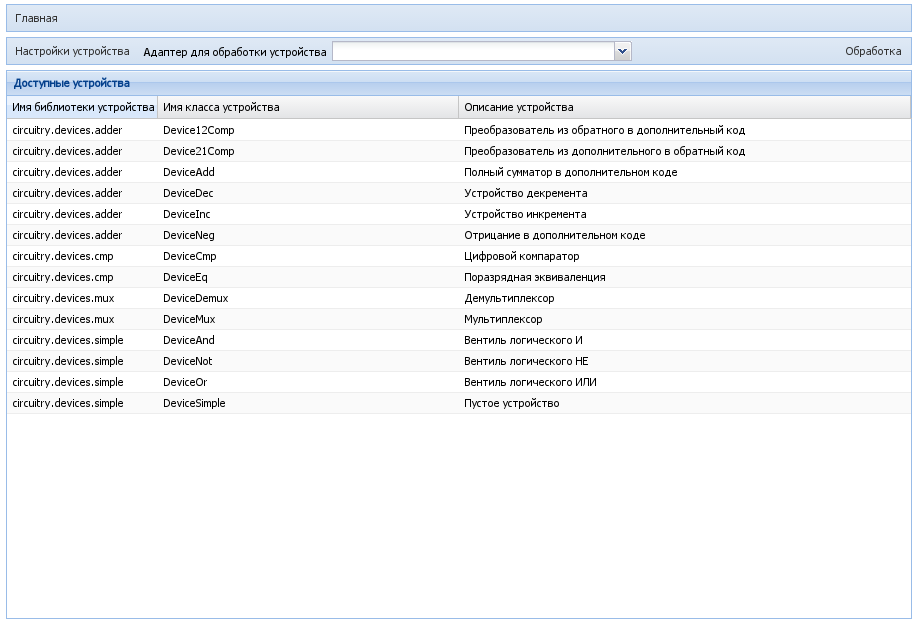
\includegraphics[width=1\linewidth]{interface_index}
\caption{Заглавная страница интерфейса пользователя}
\label{fig:interface_index}
\end{figure}

\clearpage
При выборе устройства из списка и нажатии на кнопку настройки сигналов
устройства, открывается окно настроек, где с использованием полей ввода можно
задать сигналы устройства. На рисунке~\ref{fig:interface_settings} представлено
окно настройки сигналов синтезируемого устройства.

\begin{figure}[here]
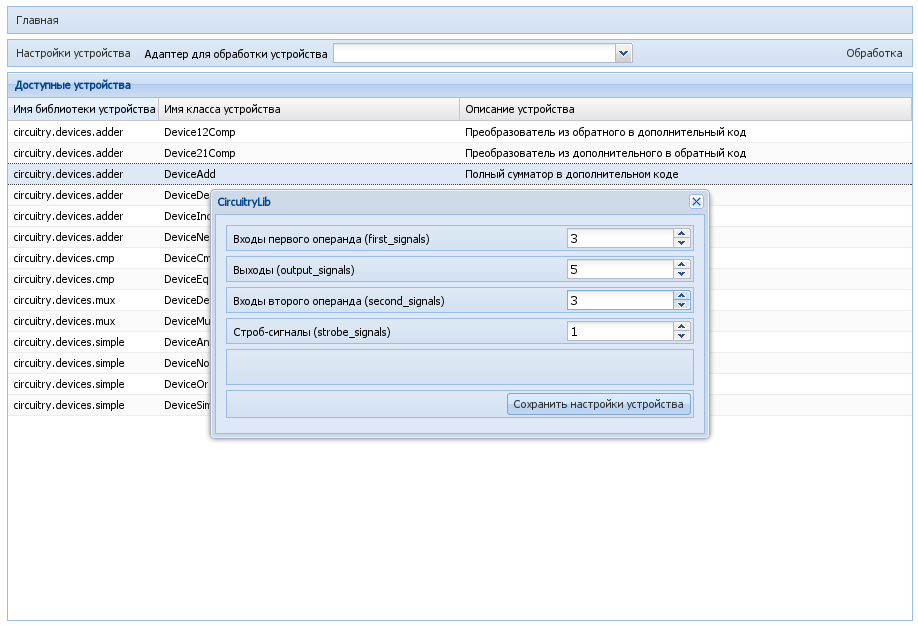
\includegraphics[width=1\linewidth]{interface_settings}
\caption{Окно настройки сигналов синтезируемого устройства}
\label{fig:interface_settings}
\end{figure}

\clearpage

После выбора адаптера, возвращающего текстовый вывод и нажатия на кнопку
обработки, открывается окно с текстовым полем, в котором находится результат
применения адаптера к синтезируемому устройству. Пример представлен на 
рисунке~\ref{fig:interface_result_text}.

\begin{figure}[here]
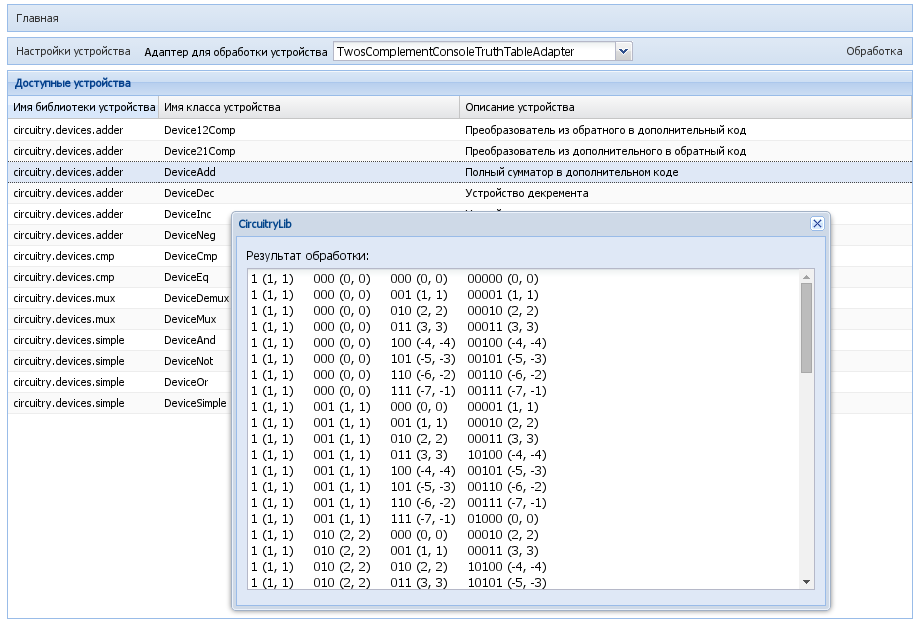
\includegraphics[width=1\linewidth]{interface_result_text}
\caption{Текстовый результат применения адаптера к синтезируемому устройству}
\label{fig:interface_result_text}
\end{figure}

\clearpage

В случае, если адаптер возвращает графический результат, окно результата будет
содержать изображение. Пример представлен на 
рисунке~\ref{fig:interface_result_graphics}.

\begin{figure}[here]
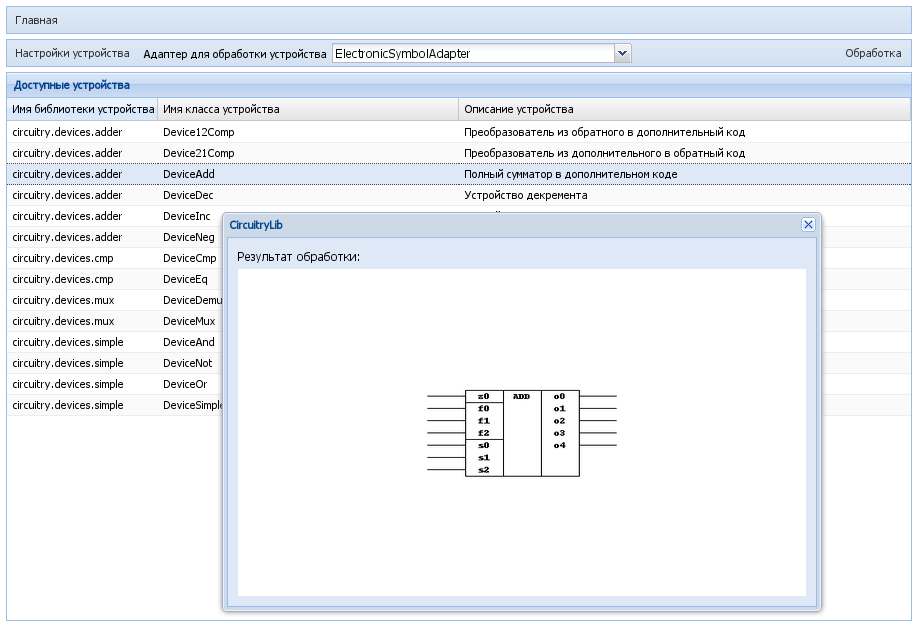
\includegraphics[width=1\linewidth]{interface_result_graphics}
\caption{Графический результат применения адаптера к синтезируемому устройству}
\label{fig:interface_result_graphics}
\end{figure}

\clearpage
\subsection{Реализованные типы синтезируемых устройств}
Следующие типы устройств, синтез которых производится созданием экземпляров
приведенных классов, были реализованы в рамках курсовой работы (в
названиях опущен префикс библиотеки -- circuitry):
\begin{itemize}[noitemsep]
  \item devices.simple.DeviceNot -- логический вентиль НЕ (инвертор) с
  возможностью поразрядной инверсии;
  \item devices.simple.DeviceAnd -- логический вентиль И (логическое умножение,
  конъюнкция);
  \item devices.simple.DeviceOr -- логический вентиль ИЛИ (логическое сложение,
  дизъюнкция);
  \item devices.mux.DeviceMux -- мультиплексор;
  \item devices.mux.DeviceDemux -- демультиплексор;
  \item devices.adder.DeviceAdd -- полный сумматор;
  \item devices.adder.DeviceInc -- инкремент;
  \item devices.adder.DeviceDec -- декремент;
  \item devices.adder.Device12Comp -- устройство преобразования из обратного
  кода в дополнительный;
  \item devices.adder.Device21Comp -- устройство преобразования из
  дополнительного кода в обратный;
  \item devices.adder.DeviceNeg -- отрицание в дополнительном коде;
  \item devices.cmp.DeviceEq -- эквиваленция (поразрядное сравнение);
  \item devices.cmp.DeviceCmp -- цифровой компаратор.
\end{itemize}

\clearpage
\subsection{Реализованные типы адаптеров}
Следующие типы адаптеров для обработки и преобразования к необходимым форматам
синтезированных устройств были реализованы в рамках проекта (в
названиях опущен префикс библиотеки -- circuitry):
\begin{itemize}[noitemsep]
  \item adapters.matlab.MatlabAdapter -- адаптер для формирования кода модели
  Simulink;
  \item adapters.matlab.extended.ExtendedMatlabAdapter -- расширенный адаптер
  для формирования кода модели Simulink, включая константы для входных сигналов
  и отображение значений выходных сигналов;
  \item adapters.visual.ElectronicSymbolAdapter -- адаптер для генерации
  условно-графического обозначения синтезируемого устройства;
  \item adapters.latex.LatexTruthTableAdapter -- адаптер для генерации таблиц
  истинности синтезируемых устройств в формате \LaTeX;
  \item adapters.latex.mux.DeviceMuxLatexTruthTableAdapter -- адаптер для
  генерации таблиц истинности мультиплексоров и демультиплексоров в формате
  \LaTeX;
  \item adapters.graph.GraphAdapter -- адаптер для представления внутренних
  структур синтезируемых устройств в виде графов библиотеки NetworkX;
  \item adapters.console.ConsoleTruthTableAdapter -- адаптер для генерации
  таблиц истинности в текстовом виде;
  \item adapters.console.TwosComplementaryConsoleTruthTableAdapter -- адаптер
  для генерации таблиц истинности в текстовом виде с отображением десятичных
  значений в обратном и дополнительном кодах.
\end{itemize}

\end{document}